
\section{Introduction} % ----------------------------------------------
Computational fluid simulations can be divided into two main categories: 
\begin{itemize}
    \item \textbf{Eulerian methods} where the space is subdivided into a grid and at each step energy transfers between adjacent cells are computed.
    \item \textbf{Lagrangian methods} which are particle-based methods, where at each step we compute the interactions between particles to update the forces that determine each particle's motion.
\end{itemize}
  Both of these methods are used to solve or approximate the Navier-Stokes equations for fluid dynamics, but for this work we will focus only on the Lagrangian methods.  \\

\noindent
The simplest formulation of the Navier-Stokes equations is the following:
\begin{align}
    \rho\frac{\partial \mathbf{u}}{\partial t} &= -\nabla p + \nu \nabla^2 \mathbf{u} + \mathbf{f} \label{eq:momentum} \\
    \nabla \cdot \mathbf{u} &= 0 \label{eq:continuity}
\end{align}
\noindent
where:
\begin{itemize}
\itemsep -1pt
    \item $\rho$ – Fluid density.
    \item $\mathbf{u}$ – Velocity field.
    \item $p$ – Pressure.
    \item $\nu$ – Kinematic viscosity.
    \item $\mathbf{f}$ – External forces (e.g., gravity).
\end{itemize}

\noindent
Eq.\eqref{eq:momentum} represents momentum conservation, while Eq.\eqref{eq:continuity} enforces the divergence of the velocity field to be zero (i.e., the volume of the fluid remains constant, which is a necessary condition for an incompressible fluid).

\subsection{SPH approximations}

Smoothed Particle Hydrodynamics (SPH) methods were introduced independently by astronomers Lucy\cite{lucy1977sph} and Gingold et al.\cite{gingold1977smph} in 1977 for approximating astrophysical fluid dynamics and, due to a lower computational cost compared to Eulerian methods, became widely adopted for real-time particle systems and fluid simulations.

\noindent
The fundamental principle of SPH methods is that, given a particle $i$ for which we want to estimate a quantity $A_i$, we can use the following equation to compute such quantity:

\begin{align}
    A_i = \sum_j{\frac{m_j}{\rho_j} \cdot A_j \cdot K(\| x_i - x_j\|, h)} \label{eq:SPH}
\end{align} 

\noindent
where:
\begin{itemize}
\itemsep -1pt
    \item \( A_i \) – Smoothed value of field quantity \( A \) at particle \( i \) (e.g., density, velocity, pressure).
    \item \( m_j \) – Mass of particle \( j \).
    \item \( \rho_j \) – Density of particle \( j \).
    \item \( A_j \) – Value of field quantity \( A \) at neighboring particle \( j \).
    \item \( K(\| x_i - x_j\|, h) \) – Smoothing kernel, weighting the influence of particle \( j \).
    \item \( \| x_i - x_j \| \) – Displacement of \( j \) with respect to \( i \).
    \item \( h \) – Smoothing length, defining the influence radius of the kernel.
\end{itemize}

\begin{figure}[ht!]
    \centering
    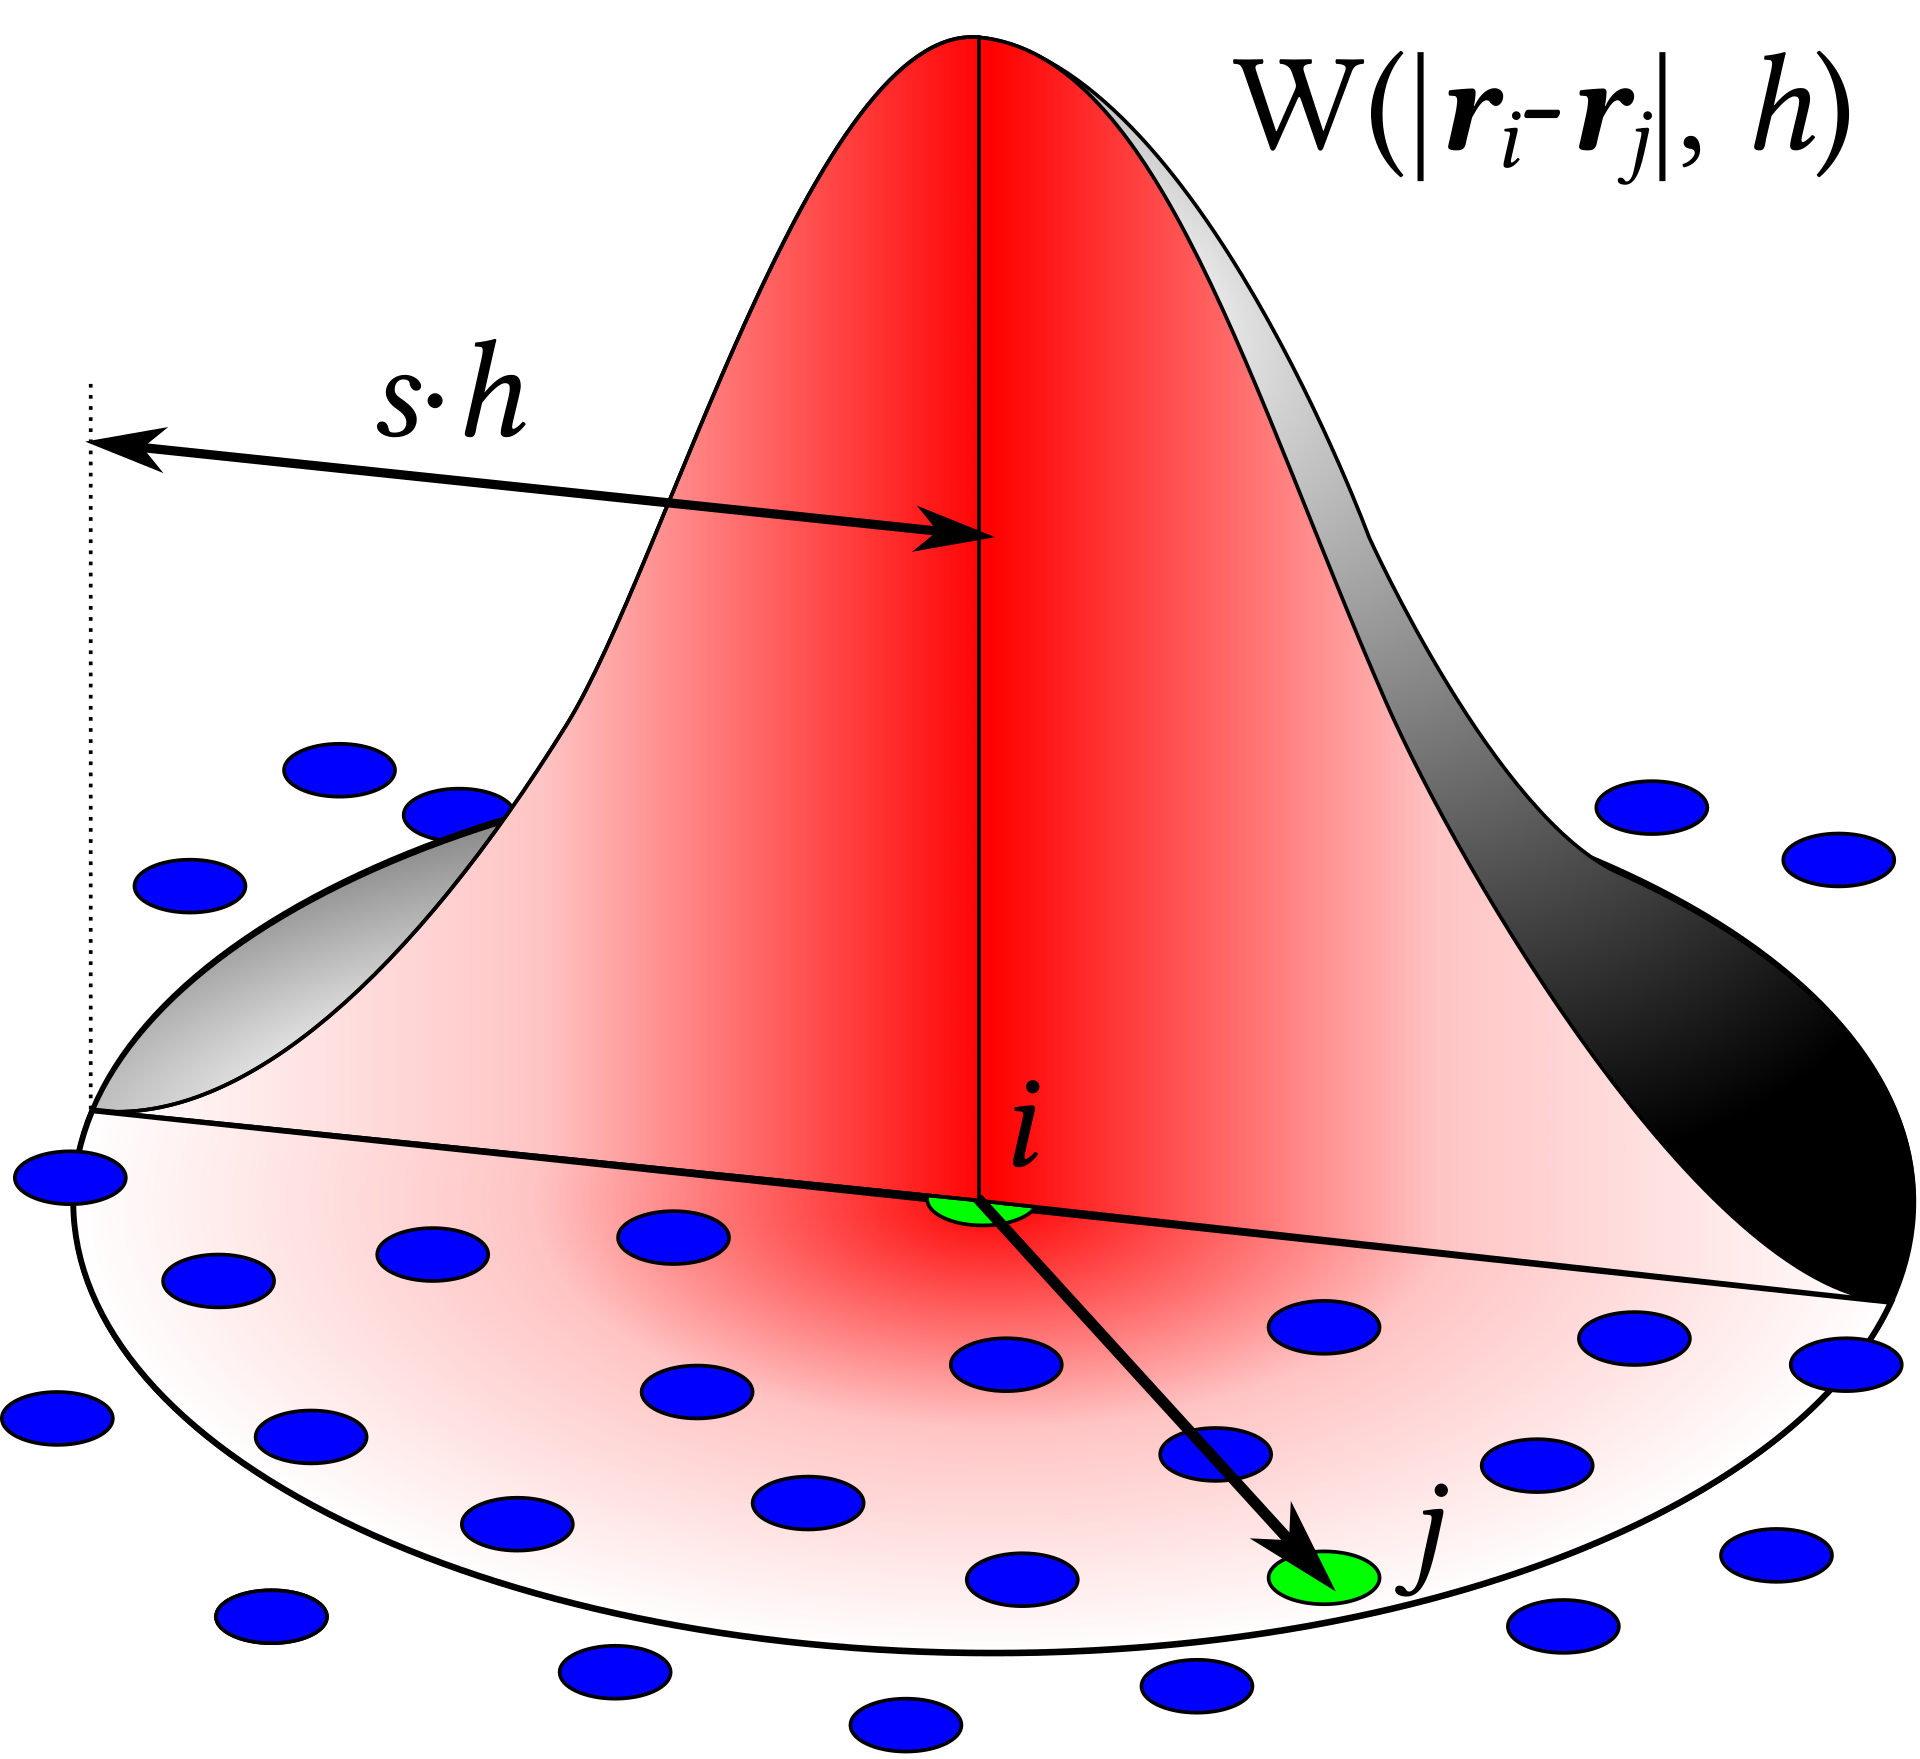
\includegraphics[height=0.35\linewidth]{images/SPH_Kernel.png}
    \caption{Visualization of the variation of a kernel function influence. Source: Wikipedia}
    \label{fig:kernelFunc}
\end{figure}

\noindent
In order to obtain an approximation that ensures physical consistency and stability, the kernel function should have at least the following properties:
\begin{itemize}
    \item \textbf{Normalization:}  
          $\int{K(\mathbf{r}, h) \, dV} = 1$ \ 
    \item \textbf{Compact Support:}  
          $ K(\mathbf{r}, h) = 0\ \text{for}\ \mathbf{r} > h $ \ 
    \item \textbf{Radial Symmetry:}  
          $ K(\mathbf{r}, h) = K(-\mathbf{r}, h) $ \ 
\end{itemize}

\noindent
In the literature, several kernel functions for density, pressure, and viscosity are proposed. For this work we used those described by Hendra in \cite{hendra2015kernels}:

\begin{itemize}
    \item \textbf{Spiky Kernel:}
    $$
        K_{spiky}(r, h) = \frac{15}{\pi h^6}
            \begin{cases}
                (h - \|r\|)^3 & 0\leq\|r\|\leq h\\
                0 & \text{otherwise} \label{eq:spiky}
            \end{cases}
    $$
    $$
        \nabla K_{spiky}(r, h) = -\frac{45}{\pi h^6}
        \begin{cases}
            \frac{r}{\|r\|}(h - \|r\|)^2 & 0\leq\|r\|\leq h\\
            0 & \text{otherwise} \label{eq:spikyGrad}
        \end{cases}
    $$
    \item \textbf{Viscosity Kernel:}
    $$
        \nabla^2 K_{viscosity}(r, h) = \frac{45}{\pi h^6}
            \begin{cases}
               (h - \|r\|) & 0\leq\|r\|\leq h\\
                0 & \text{otherwise} \label{eq:viscLaplacian}
            \end{cases}
    $$
\end{itemize}



\subsection{Approximating the Navier-Stokes equations}

Volumetric invariance (i.e., the second NS equation) is guaranteed by the fact that the number of particles in the simulation remains constant, whereas computing all the quantities needed for the first equation requires using the SPH approximation of Eq.(\ref{eq:SPH}), with some minor adjustments:
\begin{itemize}
    \item \textbf{Density ($\rho$)}: 
        \begin{align}
            \rho_i &= \sum_j{\frac{m_j}{\bcancel{\rho_j}} \bcancel{\rho_j} K_{ij}} = \sum_j{m_j K_{ij}} \label{eq:density}
        \end{align}
    \item \textbf{Pressure ($p$)}: 
        $$
            p_i = max\{k(\rho_i - \rho_0),\ \varepsilon\}
        $$
    where $k$ is a constant, $\rho_0$ is the fluid resting density and $\varepsilon$ an arbitrarily small constant.
    \item \textbf{Pressure gradient ($\nabla p$)}: 
        \begin{align}
            \nabla p_i &= \sum_j{\frac{m_j}{\rho_j}p_j \nabla K_{ij}} \approx \sum_j{\frac{m_j}{\rho_j}\frac{p_i + p_j}{2} \nabla K_{ij}} \label{eq:pGradient}
        \end{align}
    \item \textbf{Velocity Laplacian ($\nabla^2 \textbf{u}$)}: 
        \begin{align}
            \nabla^2 \textbf{u}_i &= \sum_j{\frac{m_j}{\rho_j}\textbf{u}_j \nabla^2 K_{ij}} \approx \sum_j{\frac{m_j}{\rho_j}(\textbf{u}_i - \textbf{u}_j) \nabla^2 K_{ij}}\label{eq:vLaplacian}
        \end{align}
\end{itemize}

\noindent
The last term in Eq.(\ref{eq:pGradient}) takes the average pressure of two particles, to ensure that their repulsive/attractive forces are symmetric. The same trick is used in Eq.(\ref{eq:vLaplacian}), where only the velocity difference between two particles is taken into account for the viscosity calculation.